\documentclass[tikz]{standalone}
\usetikzlibrary{arrows.meta}

\begin{document}
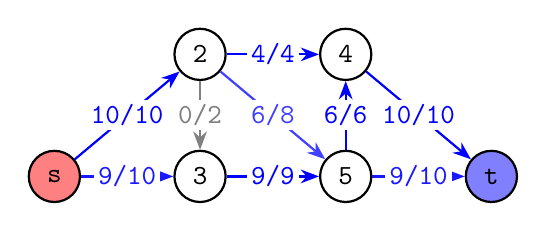
\begin{tikzpicture}[
  >=Stealth,
  font=\tt,
  vtx/.style={circle,draw,thick,minimum size=6.5mm,inner sep=0},
  lbl/.style={midway,fill=white,inner sep=1.5pt},
]
  \foreach \name/\x/\y/\fillcol in {s/0/0/red!50, 2/1.85/1.55/none, 3/1.85/0/none, 4/3.7/1.55/none, 5/3.7/0/none, t/5.55/0/blue!50}
    \node[vtx, fill=\fillcol] (\name) at (\x, \y) {\name};

  \foreach \from/\to/\lab/\col in {%
      s/2/{10/10}/blue, s/3/{9/10}/blue!90, 2/3/{0/2}/gray, 2/4/{4/4}/blue, 2/5/{6/8}/blue!75,
      3/5/{9/9}/blue, 4/t/{10/10}/blue, 5/4/{6/6}/blue, 5/t/{9/10}/blue!90}
    \draw[->, thick, \col] (\from) -- node[lbl, text=\col] {\lab} (\to);
\end{tikzpicture}
\end{document}
